\documentclass[margin=10pt]{standalone}

\usepackage[latin1]{inputenc}

\usepackage{graphicx}

\usepackage{amsmath} % nice math symbols

\usepackage{tikz}
\usetikzlibrary{positioning,calc}

\pagestyle{empty}

\newcommand{\myfont}{}

% Constants
\newcommand{\xdist}{1.5cm}
\newcommand{\xdistb}{1.2cm}
\newcommand{\xdistc}{1.0cm}
\newcommand{\xdistd}{2.5cm}
\newcommand{\xdiste}{0.3cm}
\newcommand{\xdistf}{1.5cm}
\newcommand{\ydist}{1.1cm} 
\newcommand{\ydistb}{2.8cm} 
\newcommand{\ydistc}{2.0cm} 
\newcommand{\minw}{1.0cm} % minimum width
\newcommand{\minh}{1.0cm} % minimum height
\newcommand{\textw}{2.0cm} % text width


\begin{document}
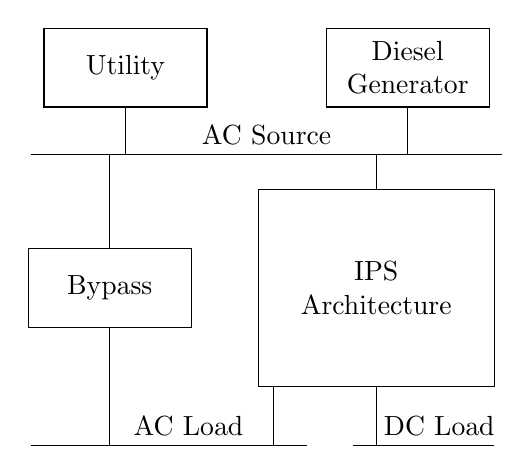
\begin{tikzpicture}[node distance = 1cm, auto] 

  %%%%%%%%%%%%%%%%%%%%%%%%%%%%%%%%%%%%%%%%%%%%%%%%%%%%%%%%%%%%%%%%%%%%%%%%%%%%%%%%%%%%%%%%%%%%%%%% 
  %%%%%%%%%%% logical scheme of IPS
  %%%%%%%%%%%%%%%%%%%%%%%%%%%%%%%%%%%%%%%%%%%%%%%%%%%%%%%%%%%%%%%%%%%%%%%%%%%%%%%%%%%%%%%%%%%%%%%% 

  
  % utility
  \node [rectangle,
  minimum width=\minw,
  minimum height=\minh,
  text centered,
  inner sep=1pt,
  text width=\textw,
  draw=black!100,
  fill=white] (utility){\myfont Utility};

  % Diesel
  \node [rectangle,
  minimum width=\minw,
  minimum height=\minh,
  text centered,
  inner sep=1pt,
  text width=2cm,
  draw=black!100,
  fill=white,
  right=\xdist of utility] (dg) {\myfont Diesel Generator};

  % bar below utility 
  \coordinate [below left=\ydist and \xdistb of utility.center] (A);
  \coordinate [below right=\ydist and \xdistb of dg.center] (B);
  \draw (A) -- (B)  node[draw=none,fill=none,font=\myfont,midway,above] {\myfont AC Source};

  % Bypass
  \node [rectangle,
  minimum width=\minw,
  minimum height=\minh,
  text centered,
  inner sep=1pt,
  text width=\textw,
  draw=black!100,
  fill=white,
  xshift=-0.2cm,
  below=\ydistb of utility.center,
  anchor=center] (bypass) {\myfont Bypass};

  % IPS
  \node [rectangle,
  minimum width=3cm,
  minimum height=2.5cm,
  text centered,
  inner sep=1pt,
  text width=1.6cm,
  draw=black!100,
  fill=white,
  xshift=-0.4cm,
  below=\ydistb of dg.center,
  anchor=center,
  label={[align=center]center:\myfont IPS\\ Architecture}] (ips) {};

  % AC load 
  \coordinate [below left=\ydistc and \xdistc of bypass.center] (C);
  \coordinate [below right=\ydistc and \xdistd of bypass.center] (D);
  \draw (C) -- (D)  node[draw=none,fill=none,font=\myfont,xshift=-1.5cm,above] {\myfont AC Load};

  % DC load 
  \coordinate [below left=\ydistc and \xdiste of ips.center] (E);
  \coordinate [below right=\ydistc and \xdistf of ips.center] (F);
  \draw (E) -- (F)  node[draw=none,fill=none,font=\myfont,xshift=-0.7cm,above] {\myfont DC Load};

  
  % line between utility and  AC Source bar
  \draw let
  \p1=(utility.center),
  \p2=(A)
  in
  (utility) -- ($(\x1, \y2)$);

  % line between Diesel Generator and  AC Source bar
  \draw let
  \p1=(dg.center),
  \p2=(A)
  in
  (dg) -- ($(\x1, \y2)$);

  % line between AC Source bar and Bypass
  \draw let
  \p1=(bypass.center),
  \p2=(A)
  in
  (bypass) -- ($(\x1, \y2)$);

  % line between AC Source bar and IPS Arch
  \draw let
  \p1=(ips.center),
  \p2=(A)
  in
  (ips) -- ($(\x1, \y2)$);

  % line between Bypass and AC Load bar
  \draw let
  \p1=(bypass.center),
  \p2=(C)
  in
  (bypass) -- ($(\x1, \y2)$);
  
  % line between IPS Arch and AC Load bar
  \draw let
  \p1=([xshift=-1.3cm]ips.south),
  \p2=(C)
  in
  ($(\x1, \y1)$) -- ($(\x1, \y2)$);

  % line between IPS Arch and DC Load bar
  \draw let
  \p1=([xshift=-0.0cm]ips.south),
  \p2=(C)
  in
  ($(\x1, \y1)$) -- ($(\x1, \y2)$);

\end{tikzpicture}

\end{document}

%%% Local Variables:
%%% mode: latex
%%% TeX-master: t
%%% End:
